\documentclass[a4 paper]{article}
% Set target color model to RGB
\usepackage[inner=1.5cm,outer=1.5cm,top=2.5cm,bottom=2.5cm]{geometry}
\usepackage{setspace}
\usepackage[rgb]{xcolor}
\usepackage{verbatim}
\usepackage{amsgen,amsmath,amstext,amsbsy,amsopn,tikz,amssymb,tkz-linknodes}
\usepackage{fancyhdr}
\usepackage[colorlinks=true, urlcolor=blue,  linkcolor=blue, citecolor=blue]{hyperref}
\usepackage[colorinlistoftodos]{todonotes}
\usepackage{rotating}
%\usetikzlibrary{through,backgrounds}
\hypersetup{%
pdfauthor={Arman Shokrollahi},%
pdftitle={Homework},%
pdfkeywords={Tikz,latex,bootstrap,uncertaintes},%
pdfcreator={PDFLaTeX},%
pdfproducer={PDFLaTeX},%
}
%\usetikzlibrary{shadows}
\usepackage[francais]{babel}
\usepackage{booktabs}
\newcommand{\ra}[1]{\renewcommand{\arraystretch}{#1}}

      \newtheorem{thm}{Theorem}[section]
      \newtheorem{prop}[thm]{Proposition}
      \newtheorem{lem}[thm]{Lemma}
      \newtheorem{cor}[thm]{Corollary}
      \newtheorem{defn}[thm]{Definition}
      \newtheorem{rem}[thm]{Remark}
      \numberwithin{equation}{section}

\newcommand{\homework}[6]{
   \pagestyle{myheadings}
   \thispagestyle{plain}
   \newpage
   \setcounter{page}{1}
   \noindent
   \begin{center}
   \framebox{
      \vbox{\vspace{2mm}
    \hbox to 6.28in { {\bf\hfill} }
       \vspace{6mm}
       \hbox to 6.28in { {\Large \hfill #1 (#2)  \hfill} }
       \vspace{6mm}
       \hbox to 6.28in { {\it Instructor: #3 \hfill Student: #5} }
       %\hbox to 6.28in { {\it TA: #4  \hfill #6}}
      \vspace{2mm}}
   }
   \end{center}
   \markboth{#5 -- #1}{#5 -- #1}
   \vspace*{4mm}
}

\newcommand{\bbF}{\mathbb{F}}
\newcommand{\bbX}{\mathbb{X}}
\newcommand{\bI}{\mathbf{I}}
\newcommand{\bX}{\mathbf{X}}
\newcommand{\bY}{\mathbf{Y}}
\newcommand{\bepsilon}{\boldsymbol{\epsilon}}
\newcommand{\balpha}{\boldsymbol{\alpha}}
\newcommand{\bbeta}{\boldsymbol{\beta}}
\newcommand{\0}{\mathbf{0}}

\begin{document}
\homework{Actividad \#11}{Apocalipsis Zombie}{Carlos Liz\'arraga Celaya}{}{Antonio Cota Rodr\'iguez}{}

\section*{Introducci\'on}

Como última actividad modelaremos diversos ataques de zombies, para el cual utilizaremos un diferentes códigos en python, los casos son los siguientes:\\

\begin{itemize}

\item Modelo basico de Zombis.
\item Modelo con Infeccion Latente.
\item Modelo con Cuarentena.
\item Modelo con Tratamiento.
\item Modelo con Erradicacion Impulsiva.\\

\end{itemize}

Seg\'un zombipedia, un zombi es una figura de leyenda, parte de la cultura popular. Es una representaci\'on de un cadaver que vuelve a revivir producto de haber sido infectado por un virus. Hay una gran variedad de zombis.\\

El siguiente ejemplo demuestra como resolver un sistema de ecuaciones diferenciales ordinaras usando SciPy, Notar que el orden  de la ecuaci\'on tambi\'en puede ser resuelta usando SciPy haciendo una transformación en el sistema de ecuaci\'on de primer orden. Es un ejemplo simple, un sistema de EDO's pueden ser utilizados como un modelo de "invasi\'on zombie", usando las ecuaciones especificados en Munz et al. 2009.\\

El sistema es dado por:

$$ dS/dt = P - BSZ - dS dZ/dt = BSZ + GR - ASZ dR/dt = dS + ASZ - GR $$

Con las siguientes notaciones:\\

\begin{itemize}

\item S: N\'umero de v\'ictimas susceptibles.
\item Z: N\'umero de zombies
\item R: N\'umero de personas asesinadas
\item P: Tasa de nacimientos
\item d: Oportunidad de muerte natural
\item B: La enfermedad zombie sea transmitida (una persona viva se convierta en zombie)
\item G: Una persona muerta sea resucitada en un zombie
\item A: El zombie sea toltamente destruido

\end{itemize}

Esto involucra resolver un sistema de ecuaciones diferenciales de primer orden dadas por : $dy/dt = f(t,t)$. Cuando $y=[S,Z,R]$.

El código que puede ser utilizado es el siguiente:

\begin{verbatim}

# zombie apocalypse modeling
import numpy as np
import matplotlib.pyplot as plt
from scipy.integrate import odeint
plt.ion()
plt.rcParams['figure.figsize'] = 10, 8

P = 0 # birth rate
d = 0.0001 # natural death percent (per day)
B = 0.0095 # transmission percent (per day)
G = 0.0001 # resurect percent (per day)
A = 0.0001 # destroy percent (per day)

# solve the system dy/dt = f(y, t)
def f(y, t):
Si = y[0]
Zi = y[1]
Ri = y[2]
# the model equations (see Munz et al. 2009)
f0 = P - B*Si*Zi - d*Si
f1 = B*Si*Zi + G*Ri - A*Si*Zi
f2 = d*Si + A*Si*Zi - G*Ri
return [f0, f1, f2]

# initial conditions
S0 = 500. # initial population
Z0 = 0 # initial zombie population
R0 = 0.05*S0 # 1% of initial pop is dead
y0 = [S0, Z0, R0]
t = np.linspace(0, 5., 1000) # time grid

# solve the DEs
soln = odeint(f, y0, t)
S = soln[:, 0]
Z = soln[:, 1]
R = soln[:, 2]

# plot results
plt.figure()
plt.plot(t, S,"Darkblue", label='Humanos vivos')
plt.plot(t, Z,"Orange", label='Zombies')
plt.xlabel('Dias despues del brote')
plt.ylabel('Poblacion')
plt.title('Apocalipsis zombie - Con el 5% de la poblacion aniquilada')
plt.legend(loc=0)


\end{verbatim}

\begin{figure}[!ht]
  \centering
      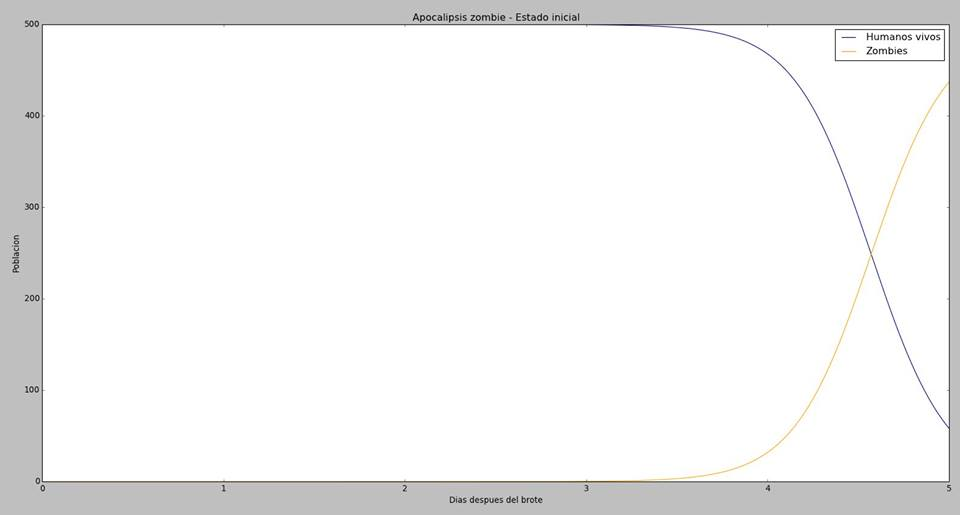
\includegraphics[width=10cm, height=6cm]{EstadoInicial.png}
  \caption{}
\end{figure}

\begin{figure}[!ht]
  \centering
      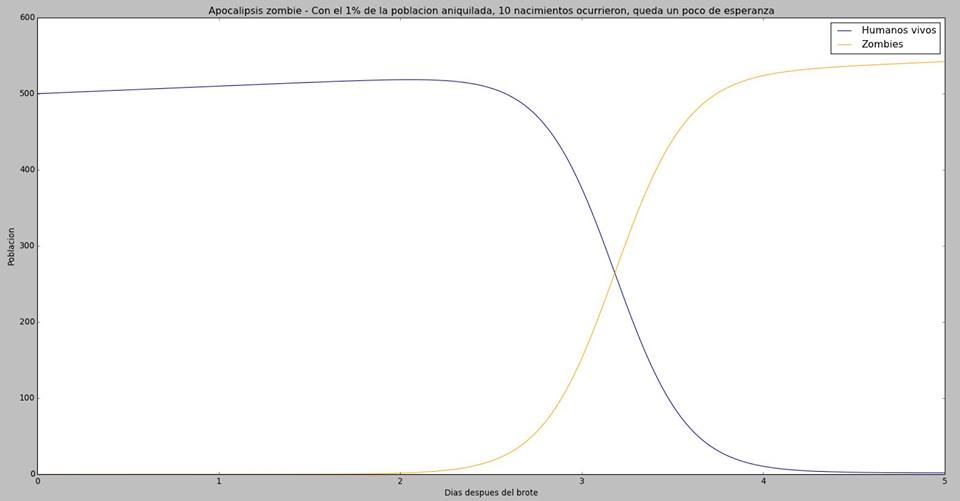
\includegraphics[width=10cm, height=6cm]{Aniquilada1.png}
  \caption{}
\end{figure}


Este es el modelo base que se nos brind\'o. Ahora hay que modelar los casos mencionados arriba.\\

El siguiente caso es para el {\bf Modelo con Infeccion Latente}\\

\begin{verbatim}
# zombie apocalypse modeling
import numpy as np
import matplotlib.pyplot as plt
from scipy.integrate import odeint
plt.ion()
plt.rcParams['figure.figsize'] = 10, 8

P = 0 # birth rate
d = 0.0001 # natural death percent (per day)
B = 0.0095 # transmission percent (per day)
G = 0.0001 # resurect percent (per day)
A = 0.0001 # destroy percent (per day)
rho = 0.3

# solve the system dy/dt = f(y, t)
def f(y, t):
Si = y[0]
Ii = y[1]
Zi = y[2]
Ri = y[3]
# the model equations (see Munz et al. 2009)
f0 = P - B*Si*Zi - d*Si
f1 = B*Si*Zi - rho*Ii - d*Ii
f2 = rho*Ii + G*Ri - A*Si*Zi
f3 = d*Si + d*Ii + A*Si*Zi - G*Ri
return [f0, f1, f2, f3]

# initial conditions
S0 = 500. # initial population
I0 = 1
Z0 = 0 # initial zombie population
R0 = 0 # 1% of initial pop is dead
y0 = [S0, I0, Z0, R0]
t = np.linspace(0, 20, 1000) # time grid

# solve the DEs
soln = odeint(f, y0, t)
S = soln[:, 0]
I = soln[:, 1]
Z = soln[:, 2]
R = soln[:, 3]

# plot results
plt.figure()
plt.plot(t, S,"Darkblue", label='Humanos vivos')
plt.plot(t, Z,"Orange", label='Zombies')
plt.xlabel('Dias despues del brote')
plt.ylabel('Poblacion')
plt.title('Apocalipsis zombie - Infeccion latente')
plt.legend(loc=0)
\end{verbatim}

\begin{figure}[!ht]
  \centering
      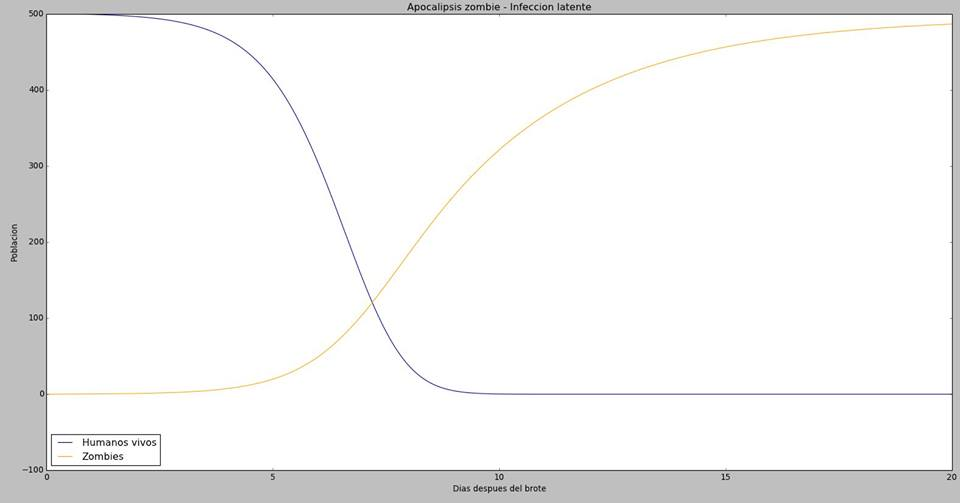
\includegraphics[width=10cm, height=6cm]{Infeccionlatente.png}
  \caption{}
\end{figure}

Ahora para el caso de {\bf Modo Cuarentena}:

\begin{verbatim}
# zombie apocalypse modeling
import numpy as np
import matplotlib.pyplot as plt
from scipy.integrate import odeint
plt.ion()
plt.rcParams['figure.figsize'] = 10, 8

P = 0 # birth rate
d = 0.0001 # natural death percent (per day)
B = 0.0095 # transmission percent (per day)
G = 0.0001 # resurect percent (per day)
A = 0.0001 # destroy percent (per day)
rho = 0.3
k = 0.001
sigma = 0.0009
Ga = 0.004

# solve the system dy/dt = f(y, t)
def f(y, t):
Si = y[0]
Ii = y[1]
Zi = y[2]
Ri = y[3]
Qi = y[4]
# the model equations (see Munz et al. 2009)
f0 = P - B*Si*Zi - d*Si
f1 = B*Si*Zi - rho*Ii - d*Ii - k*Ii
f2 = rho*Ii + G*Ri - A*Si*Zi - sigma*Zi
f3 = d*Si + d*Ii + A*Si*Zi - G*Ri + Ga* Qi
f4 = k*Ii + sigma*Zi - Ga*Qi
return [f0, f1, f2, f3, f4]

# initial conditions
S0 = 500. # initial population
I0 = 100
Z0 = 0 # initial zombie population
Q0 = 130
R0 = 0 # 1% of initial pop is dead
y0 = [S0, I0, Z0, R0, Q0]
t = np.linspace(0, 20, 1000) # time grid

# solve the DEs
soln = odeint(f, y0, t)
S = soln[:, 0]
I = soln[:, 1]
Z = soln[:, 2]
R = soln[:, 3]
Q = soln[:, 4]

# plot results
plt.figure()
plt.plot(t, S,"Darkblue", label='Humanos vivos')
plt.plot(t, Z,"Orange", label='Zombies')
plt.xlabel('Dias despues del brote')
plt.ylabel('Poblacion')
plt.title('Apocalipsis zombie - Modo cuarentena')
plt.legend(loc=0)
\end{verbatim}

\begin{figure}[!ht]
  \centering
      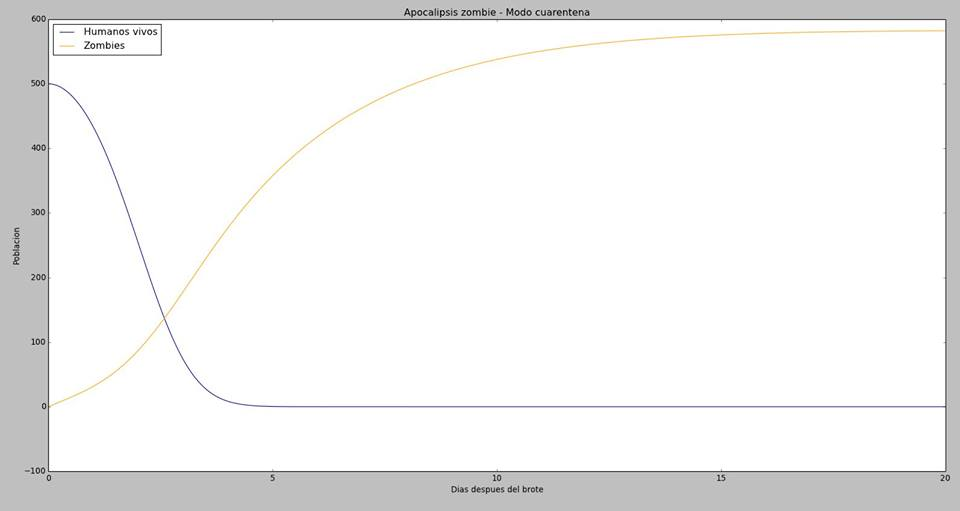
\includegraphics[width=10cm, height=6cm]{Modocuarentena.png}
  \caption{}
\end{figure}

Y por \'ultimo el caso de {\bf Modo Tratamiento}:

\begin{verbatim}

# zombie apocalypse modeling
import numpy as np
import matplotlib.pyplot as plt
from scipy.integrate import odeint
plt.ion()
plt.rcParams['figure.figsize'] = 10, 8

P = 0 # birth rate
d = 0.0001 # natural death percent (per day)
B = 0.0095 # transmission percent (per day)
G = 0.0001 # resurect percent (per day)
A = 0.0001 # destroy percent (per day)
rho = 0.3
C = 0.1 

# solve the system dy/dt = f(y, t)
def f(y, t):
Si = y[0]
Ii = y[1]
Zi = y[2]
Ri = y[3]
# the model equations (see Munz et al. 2009)
f0 = P - B*Si*Zi - d*Si + C*Zi
f1 = B*Si*Zi - rho*Ii - d*Ii
f2 = rho*Ii + G*Ri - A*Si*Zi -C*Zi
f3 = d*Si + d*Ii + A*Si*Zi - G*Ri
return [f0, f1, f2, f3]

# initial conditions
S0 = 500. # initial population
I0 = 50
Z0 = 0 # initial zombie population
R0 = 0 # 1% of initial pop is dead
y0 = [S0, I0, Z0, R0]
t = np.linspace(0, 20, 1000) # time grid

# solve the DEs
soln = odeint(f, y0, t)
S = soln[:, 0]
I = soln[:, 1]
Z = soln[:, 2]
R = soln[:, 3]

# plot results
plt.figure()
plt.plot(t, S,"Darkblue", label='Humanos vivos')
plt.plot(t, Z,"Orange", label='Zombies')
plt.xlabel('Dias despues del brote')
plt.ylabel('Poblacion')
plt.title('Apocalipsis zombie - Modo tratamiento')
plt.legend(loc=0)

\end{verbatim}
\newpage
\begin{figure}[!ht]
  \centering
      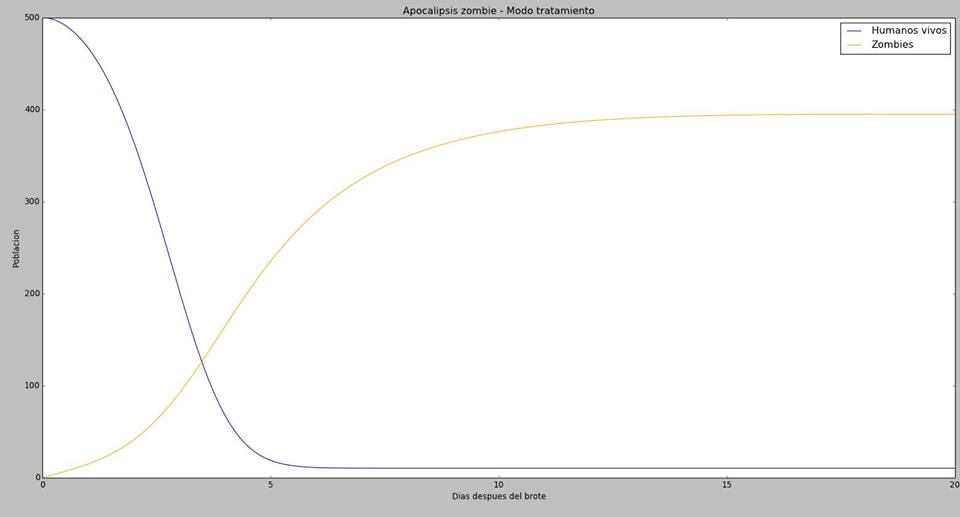
\includegraphics[width=10cm, height=6cm]{tratamiento.png}
  \caption{}
\end{figure}



\end{document}